\section{Observations and Calculations}
	\subsection{Frequency dependence of Dielectric Constant/Capacitance}
		\subsubsection{$BaTiO_3$}
			\begin{itemize}
				\item Permittivity of Space $(\epsilon_0) = 8.85\times10^{-3} pFmm^{-1}$
				\item Thickness $(t) = 1.45 mm$
				\item Diameter = $10 mm$
				\item Area $(A) = 78.53 mm^2$
				\item $R_3 = 3 k\ohm$
				\item $C_2 = 1000 pF$
				\item $C =\frac{\epsilon A}{t}$
			\end{itemize}

			\begin{table}[h]
	\centering
	\begin{tabular}{|c|c|c|c|}
	\hline
	\textbf{\begin{tabular}[c]{@{}c@{}}Angle\\ $(\theta)$\end{tabular}} & \textbf{Time (s)} & \textbf{Counts} & \textbf{\begin{tabular}[c]{@{}c@{}}Counts per\\ second $N(\theta)$\end{tabular}} \\ \hline
	\multirow{5}{*}{25} & \multirow{5}{*}{600} & 133 & \multirow{5}{*}{0.225} \\ \cline{3-3}
	 &  & 140 &  \\ \cline{3-3}
	 &  & 127 &  \\ \cline{3-3}
	 &  & 137 &  \\ \cline{3-3}
	 &  & 138 &  \\ \hline
	\multirow{5}{*}{20} & \multirow{5}{*}{200} & 164 & \multirow{5}{*}{0.940} \\ \cline{3-3}
	 &  & 198 &  \\ \cline{3-3}
	 &  & 186 &  \\ \cline{3-3}
	 &  & 195 &  \\ \cline{3-3}
	 &  & 197 &  \\ \hline
	\multirow{5}{*}{15} & \multirow{5}{*}{100} & 311 & \multirow{5}{*}{2.929} \\ \cline{3-3}
	 &  & 276 &  \\ \cline{3-3}
	 &  & 277 &  \\ \cline{3-3}
	 &  & 311 &  \\ \cline{3-3}
	 &  & 290 &  \\ \hline
	\multirow{5}{*}{10} & \multirow{5}{*}{100} & 1726 & \multirow{5}{*}{17.626} \\ \cline{3-3}
	 &  & 1811 &  \\ \cline{3-3}
	 &  & 1713 &  \\ \cline{3-3}
	 &  & 1754 &  \\ \cline{3-3}
	 &  & 1809 &  \\ \hline
	\multirow{5}{*}{5} & \multirow{5}{*}{100} & 2931 & \multirow{5}{*}{29.286} \\ \cline{3-3}
	 &  & 2938 &  \\ \cline{3-3}
	 &  & 2912 &  \\ \cline{3-3}
	 &  & 2931 &  \\ \cline{3-3}
	 &  & 2931 &  \\ \hline
	\multirow{5}{*}{-5} & \multirow{5}{*}{100} & 2934 & \multirow{5}{*}{29.343} \\ \cline{3-3}
	 &  & 2933 &  \\ \cline{3-3}
	 &  & 2935 &  \\ \cline{3-3}
	 &  & 2935 &  \\ \cline{3-3}
	 &  & 2935 &  \\ \hline
	\multirow{5}{*}{-10} & \multirow{5}{*}{100} & 1751 & \multirow{5}{*}{17.824} \\ \cline{3-3}
	 &  & 1778 &  \\ \cline{3-3}
	 &  & 1831 &  \\ \cline{3-3}
	 &  & 1787 &  \\ \cline{3-3}
	 &  & 1766 &  \\ \hline
	\multirow{5}{*}{-15} & \multirow{5}{*}{100} & 291 & \multirow{5}{*}{2.940} \\ \cline{3-3}
	 &  & 294 &  \\ \cline{3-3}
	 &  & 289 &  \\ \cline{3-3}
	 &  & 290 &  \\ \cline{3-3}
	 &  & 306 &  \\ \hline
	\multirow{5}{*}{-20} & \multirow{5}{*}{200} & 210 & \multirow{5}{*}{1.009} \\ \cline{3-3}
	 &  & 194 &  \\ \cline{3-3}
	 &  & 211 &  \\ \cline{3-3}
	 &  & 201 &  \\ \cline{3-3}
	 &  & 194 &  \\ \hline
	\multirow{5}{*}{-25} & \multirow{5}{*}{600} & 133 & \multirow{5}{*}{0.225} \\ \cline{3-3}
	 &  & 140 &  \\ \cline{3-3}
	 &  & 127 &  \\ \cline{3-3}
	 &  & 135 &  \\ \cline{3-3}
	 &  & 141 &  \\ \hline
	\end{tabular}
	\caption{Table for $N(\theta)$ for 5mm thick Gold foil}
	\label{tab:1}
\end{table}
			\begin{figure}[H]
				\centering
				\label{graph:1}
				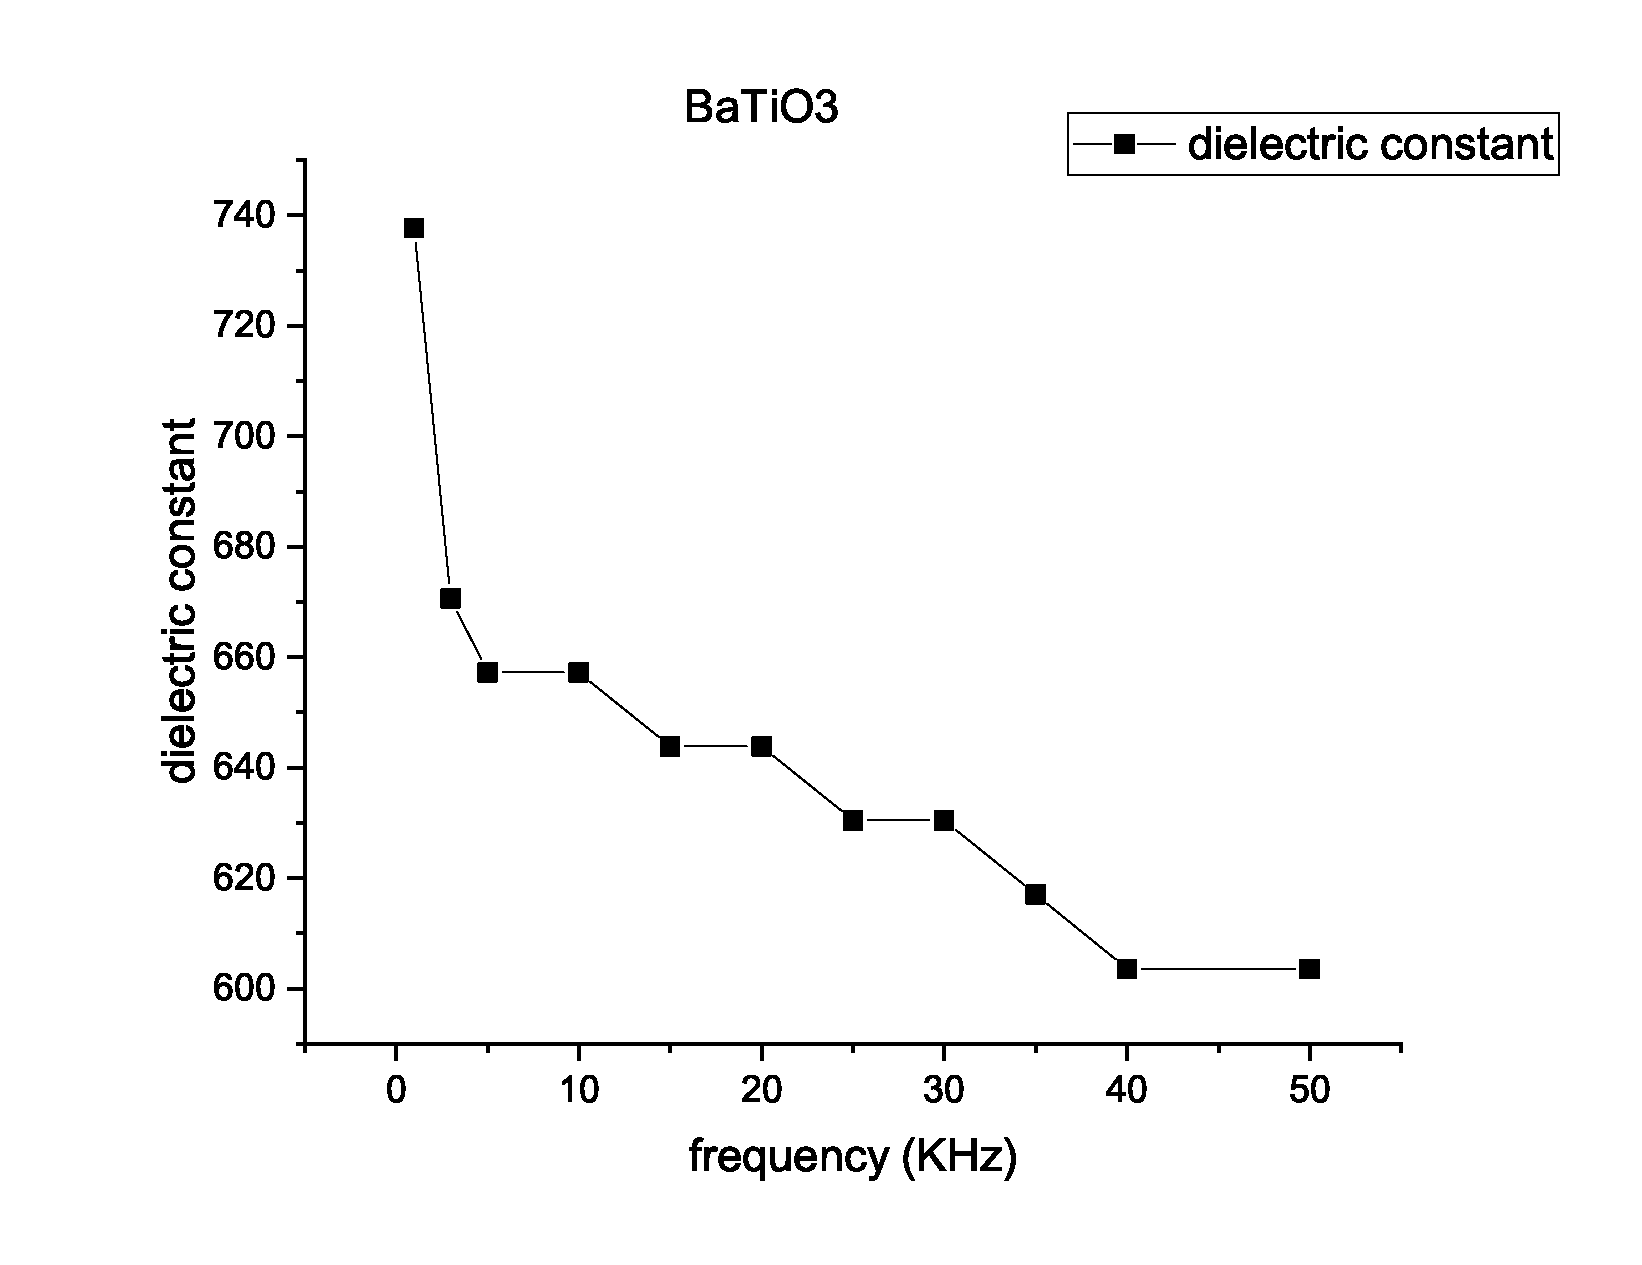
\includegraphics[width=0.8\columnwidth]{images/G1.eps}
				\caption{Dielectric constant vs frequency graph for $BaTiO_3$}
			\end{figure}
			\begin{figure}[H]
				\centering
				\label{graph:2}
				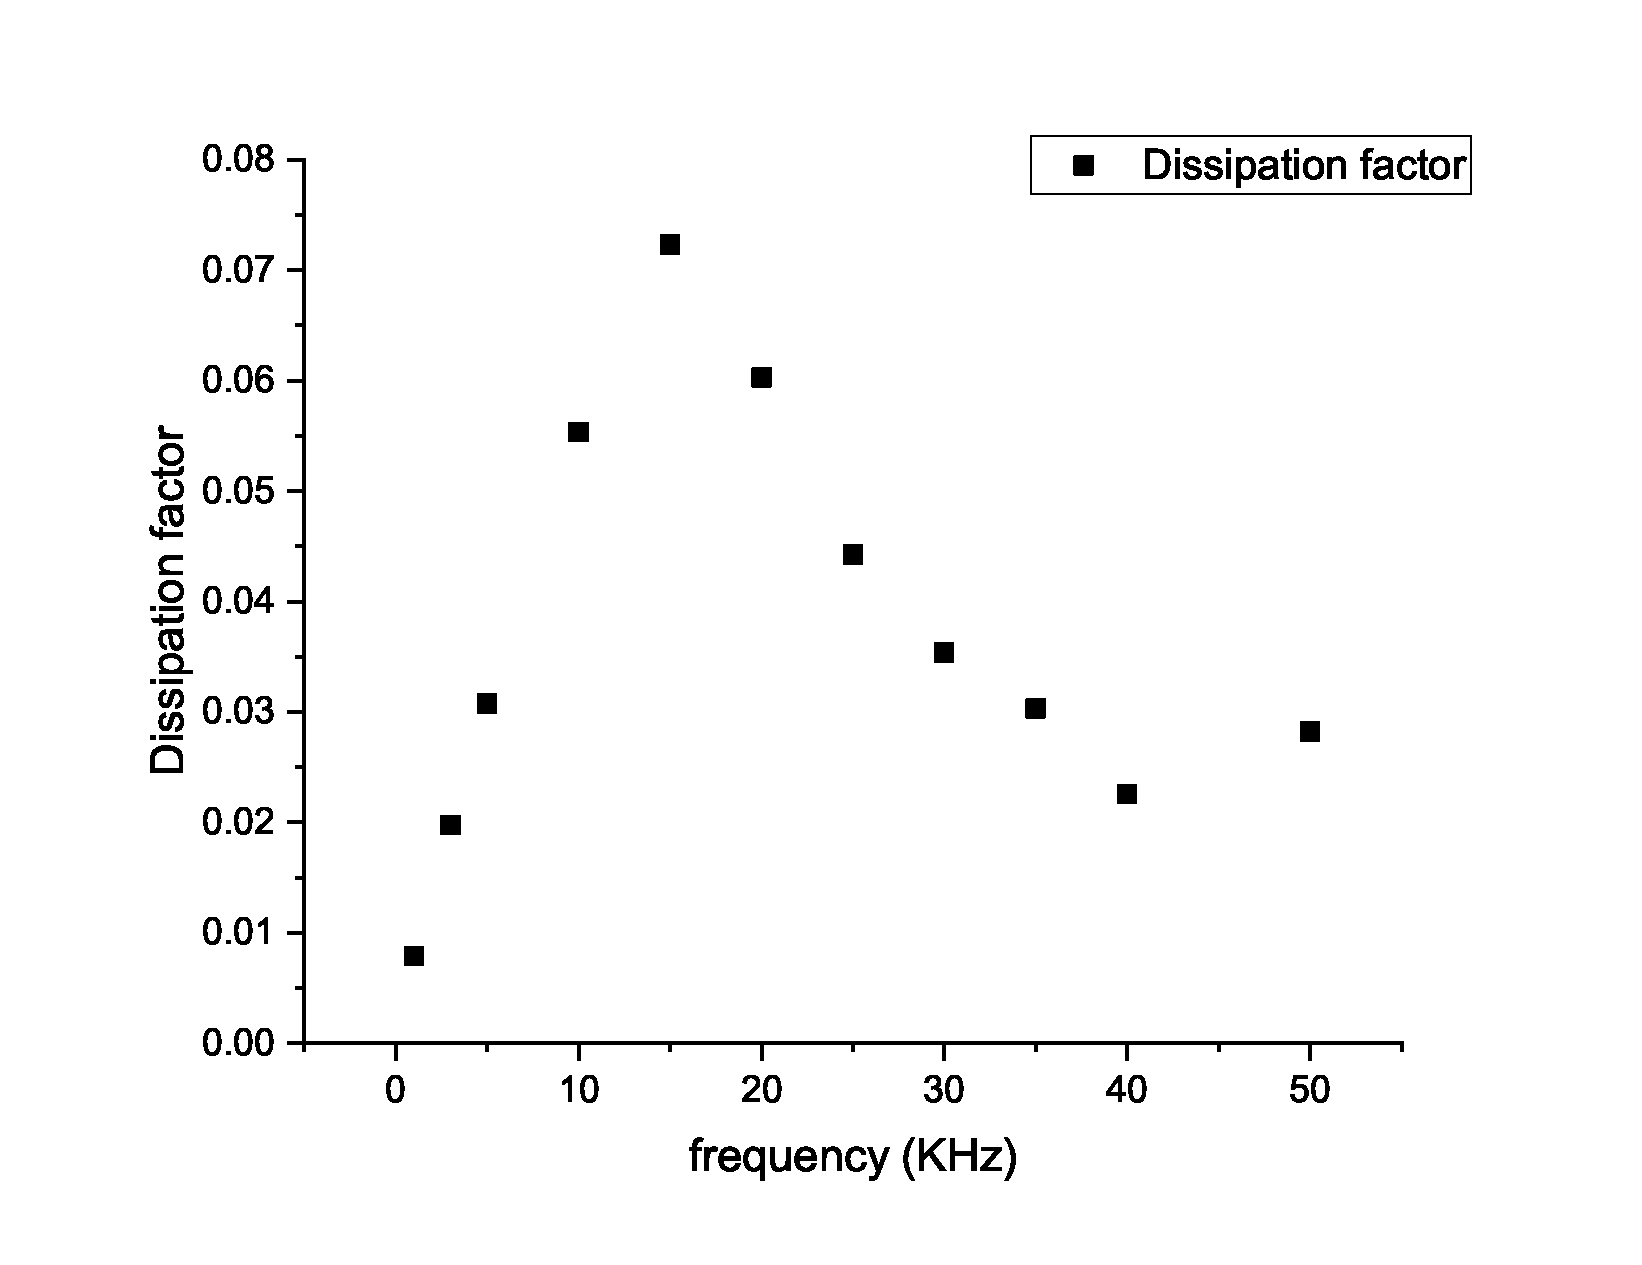
\includegraphics[width=0.8\columnwidth]{images/g2.eps}
				\caption{Dissipation factor vs frequency graph for $BaTiO_3$}
			\end{figure}
		\subsubsection{Multi-layer Ceramic Capacitor (MLCC)}

			\begin{table}[H]
    \centering
    \begin{tabular}{|c|c|c|c|}
        \hline
        $V_{DC}$ & $V_{DUT}$ & $V_{OUT}$ & $C_{DUT}$   \\ \hline
        0        & 0.074     & 0.459     & 127.837 \\
        0.1      & 0.109     & 0.451     &  85.276 \\
        0.2      & 0.232     & 0.447     &  39.709 \\
        0.3      & 0.299     & 0.438     &  30.191 \\
        0.4      & 0.389     & 0.432     &  22.888 \\
        0.5      & 0.463     & 0.432     &  19.230 \\
        0.6      & 0.564     & 0.426     &  15.567 \\
        0.7      & 0.662     & 0.420     &  13.075 \\
        0.8      & 0.760     & 0.435     &  11.796 \\
        0.9      & 0.846     & 0.430     &  10.475 \\
        1        & 0.941     & 0.426     &   9.330 \\
        1.1      & 1.058     & 0.427     &   8.318 \\
        1.2      & 1.174     & 0.422     &   7.408 \\
        1.3      & 1.267     & 0.418     &   6.799 \\
        1.4      & 1.357     & 0.416     &   6.318 \\
        1.5      & 1.464     & 0.412     &   5.800 \\
        1.6      & 1.559     & 0.409     &   5.406 \\ \hline
    \end{tabular}
    \caption{Data for light condition}
    \label{tab:2}
\end{table}
			\begin{figure}[H]
				\centering
				\label{graph:3}
				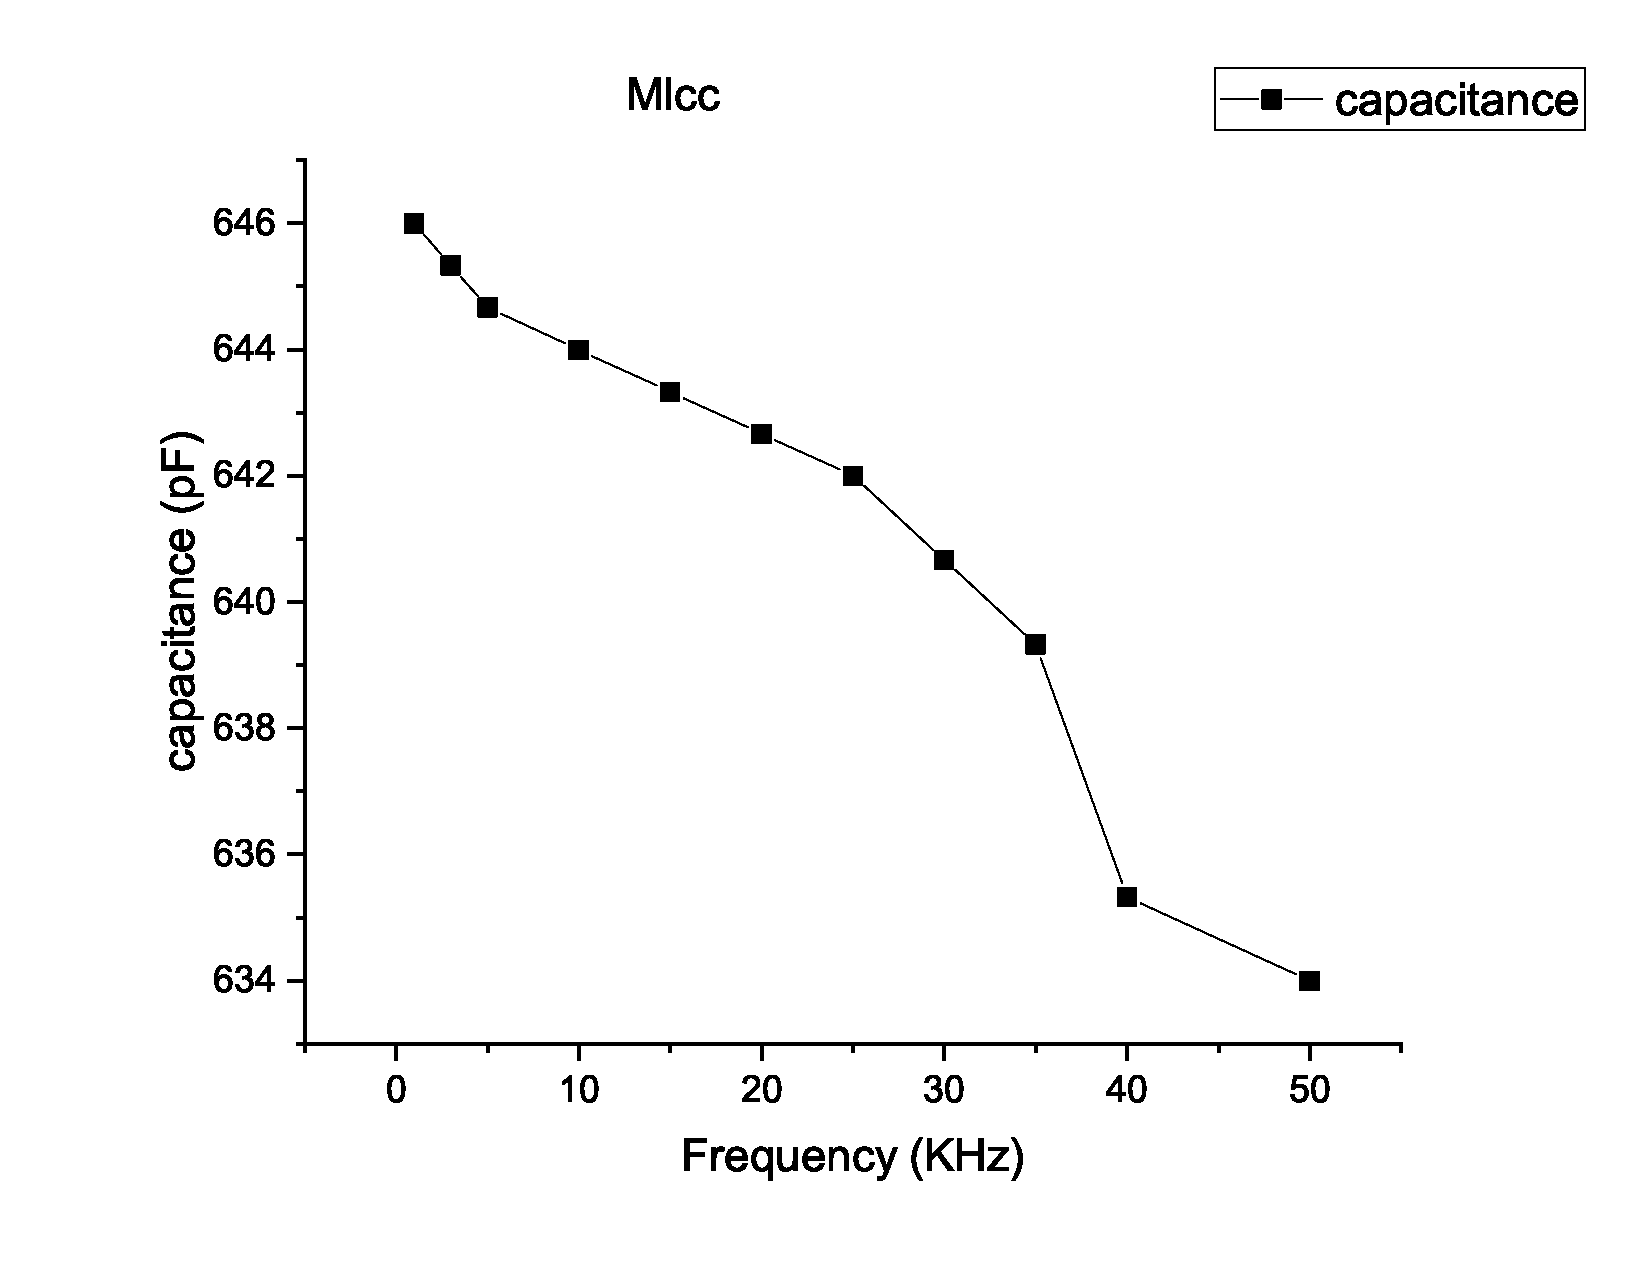
\includegraphics[width=0.8\columnwidth]{images/g3.eps}
				\caption{capacitance vs frequency graph for MLCC}
			\end{figure}


		\subsubsection{Disc Ceramic Capacitor (DCC)}

			\begin{table}[]
	\centering
	\begin{tabular}{|l|l|}
	\hline
		H(gauss) & V(mV) \\ \hline
		2390 & -0.061 \\ \hline
		2540 & -0.062 \\ \hline
		3160 & -0.063 \\ \hline
		3480 & -0.064 \\ \hline
		4200 & -0.065 \\ \hline
		4500 & -0.066 \\ \hline
		4780 & -0.067 \\ \hline
		5200 & -0.068 \\ \hline
		5180 & -0.069 \\ \hline
	\end{tabular}
	\caption{Magnetoresistance Data for $I=101.0mA$}
	\label{tab:mag2}
\end{table}
			\begin{figure}[H]
				\centering
				\label{graph:4}
				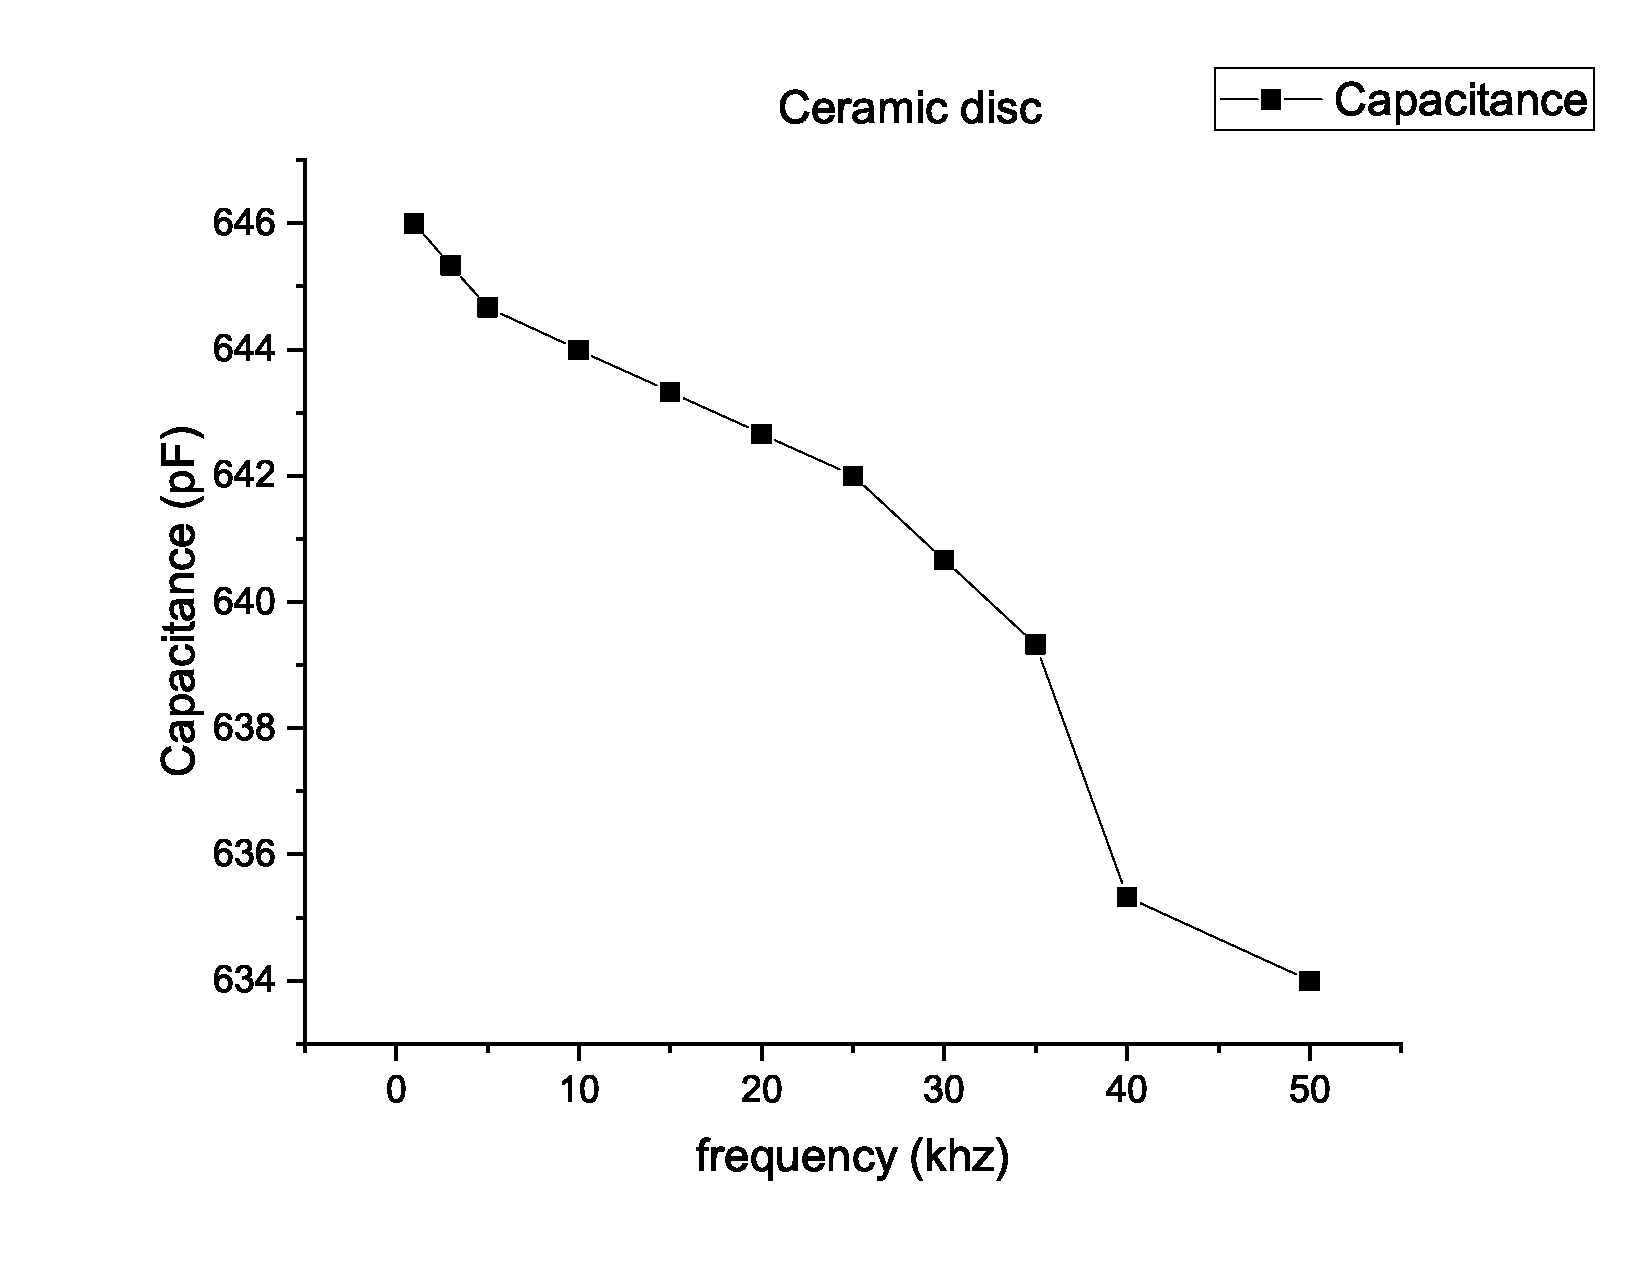
\includegraphics[width=0.8\columnwidth]{images/g4.eps}
				\caption{capacitance vs frequency graph for DCC}
			\end{figure}
	\subsection{Study of the temperature dependence of dielectric constant at different frequencies using Barium Titanate Sample}

		\begin{table}[h]
	\centering
	\resizebox{\columnwidth}{!}{%
		\begin{tabular}{|c|c|c|c|c|c|}
			\hline
			\textbf{Source}                      & \textbf{Distance (cm)} & \textbf{Counts} & \textbf{Corrected Counts} & \textbf{Average}         & \multicolumn{1}{l|}{\textbf{CPS}} \\ \hline
			\multirow{3}{*}{\textbf{$Cs^{137}$}} & \multirow{3}{*}{10}    & 738             & 655                       & \multirow{3}{*}{670.667} & \multirow{3}{*}{11.178}           \\ \cline{3-4}
			                                     &                        & 766             & 683                       &                          &                                   \\ \cline{3-4}
			                                     &                        & 757             & 674                       &                          &                                   \\ \hline
			\multirow{3}{*}{\textbf{$Tl^{204}$}} & \multirow{3}{*}{2}     & 2306            & 2223                      & \multirow{3}{*}{2224}    & \multirow{3}{*}{37.067}           \\ \cline{3-4}
			                                     &                        & 2309            & 2226                      &                          &                                   \\ \cline{3-4}
			                                     &                        & 2306            & 2223                      &                          &                                   \\ \hline
		\end{tabular}%
	}
	\caption{Efficiency Data}
	\label{tab:4}
\end{table}
		\begin{table}[H]
    \centering
    \begin{tabular}{|l|l|l|l|}
    \hline
        Operating voltage & ~ & FMWH & Resolution(\%) \\ \hline
        500 & ~ & 0.41734 & 10.38 \\ \hline
        550 & ~ & 0.39714 & 10.18 \\ \hline
        600 & ~ & 0.3943 & 10.48 \\ \hline
        650 & ~ & 0.40354 & 10.29 \\ \hline
    \end{tabular}
    \caption{Operating voltage vs FMWH and resolution}
    \label{tab:resolution}
\end{table}
		\begin{table}[H]
    \centering
    \begin{tabular}{|c|c|c|c|c|}
        \hline
        Temperature & R       & c(pF) & C1     & $\epsilon$ \\ \hline
        $^{\circ}$C & K$\ohm$ & pF    & pF     & ~          \\ \hline
        50          & 1.08    & 100   & 360.00 & 724.35     \\ \hline
        60          & 1.14    & 100   & 380.00 & 764.59     \\ \hline
        70          & 1.18    & 100   & 393.33 & 791.42     \\ \hline
        80          & 1.142   & 100   & 380.67 & 765.93     \\ \hline
        90          & 1.172   & 100   & 390.67 & 786.05     \\ \hline
        100         & 1.186   & 100   & 395.33 & 795.44     \\ \hline
        110         & 1.224   & 100   & 408.00 & 820.93     \\ \hline
        120         & 1.266   & 100   & 422.00 & 849.09     \\ \hline
        130         & 1.342   & 100   & 447.33 & 900.07     \\ \hline
        140         & 1.39    & 100   & 463.33 & 932.26     \\ \hline
        150         & 1.36    & 100   & 453.33 & 912.14     \\ \hline
        160         & 1.28    & 50    & 426.67 & 858.48     \\ \hline
        170         & 1.2     & 50    & 400.00 & 804.83     \\ \hline
        180         & 1.14    & 50    & 380.00 & 764.59     \\ \hline
    \end{tabular}
    \caption{observed capacitance value for $BaTiO_3$ at different temperature at 25kHz}
    \label{tab:6}
\end{table}
		\begin{table}[H]
    \centering
    \begin{tabular}{|c|c|c|c|c|}
        \hline
        Temperature & R       & c(pF) & C1     & $\epsilon$ \\ \hline
        $^{\circ}$C & K$\ohm$ & pF    & pF     & ~          \\ \hline
        50          & 1.07    & 50    & 356.67 & 717.63     \\ \hline
        60          & 1.08    & 50    & 360.00 & 724.34     \\ \hline
        70          & 1.09    & 50    & 363.33 & 731.05     \\ \hline
        80          & 1.13    & 50    & 376.67 & 757.88     \\ \hline
        90          & 1.16    & 50    & 386.67 & 778.00     \\ \hline
        100         & 1.18    & 50    & 392.00 & 788.73     \\ \hline
        110         & 1.21    & 50    & 403.33 & 811.53     \\ \hline
        120         & 1.25    & 50    & 418.00 & 841.04     \\ \hline
        130         & 1.32    & 50    & 439.33 & 883.97     \\ \hline
        140         & 1.36    & 50    & 453.33 & 912.13     \\ \hline
        150         & 1.32    & 50    & 440.00 & 885.31     \\ \hline
        160         & 1.20    & 50    & 400.00 & 804.82     \\ \hline
        170         & 1.18    & 50    & 393.33 & 791.41     \\ \hline
        180         & 1.14    & 50    & 380.00 & 764.58     \\ \hline
    \end{tabular}
    \caption{observed capacitance value for $BaTiO_3$ at different temperature at 35kHz}
    \label{tab:7}
\end{table}
		\begin{figure}[H]
			\centering
			\label{graph:5}
			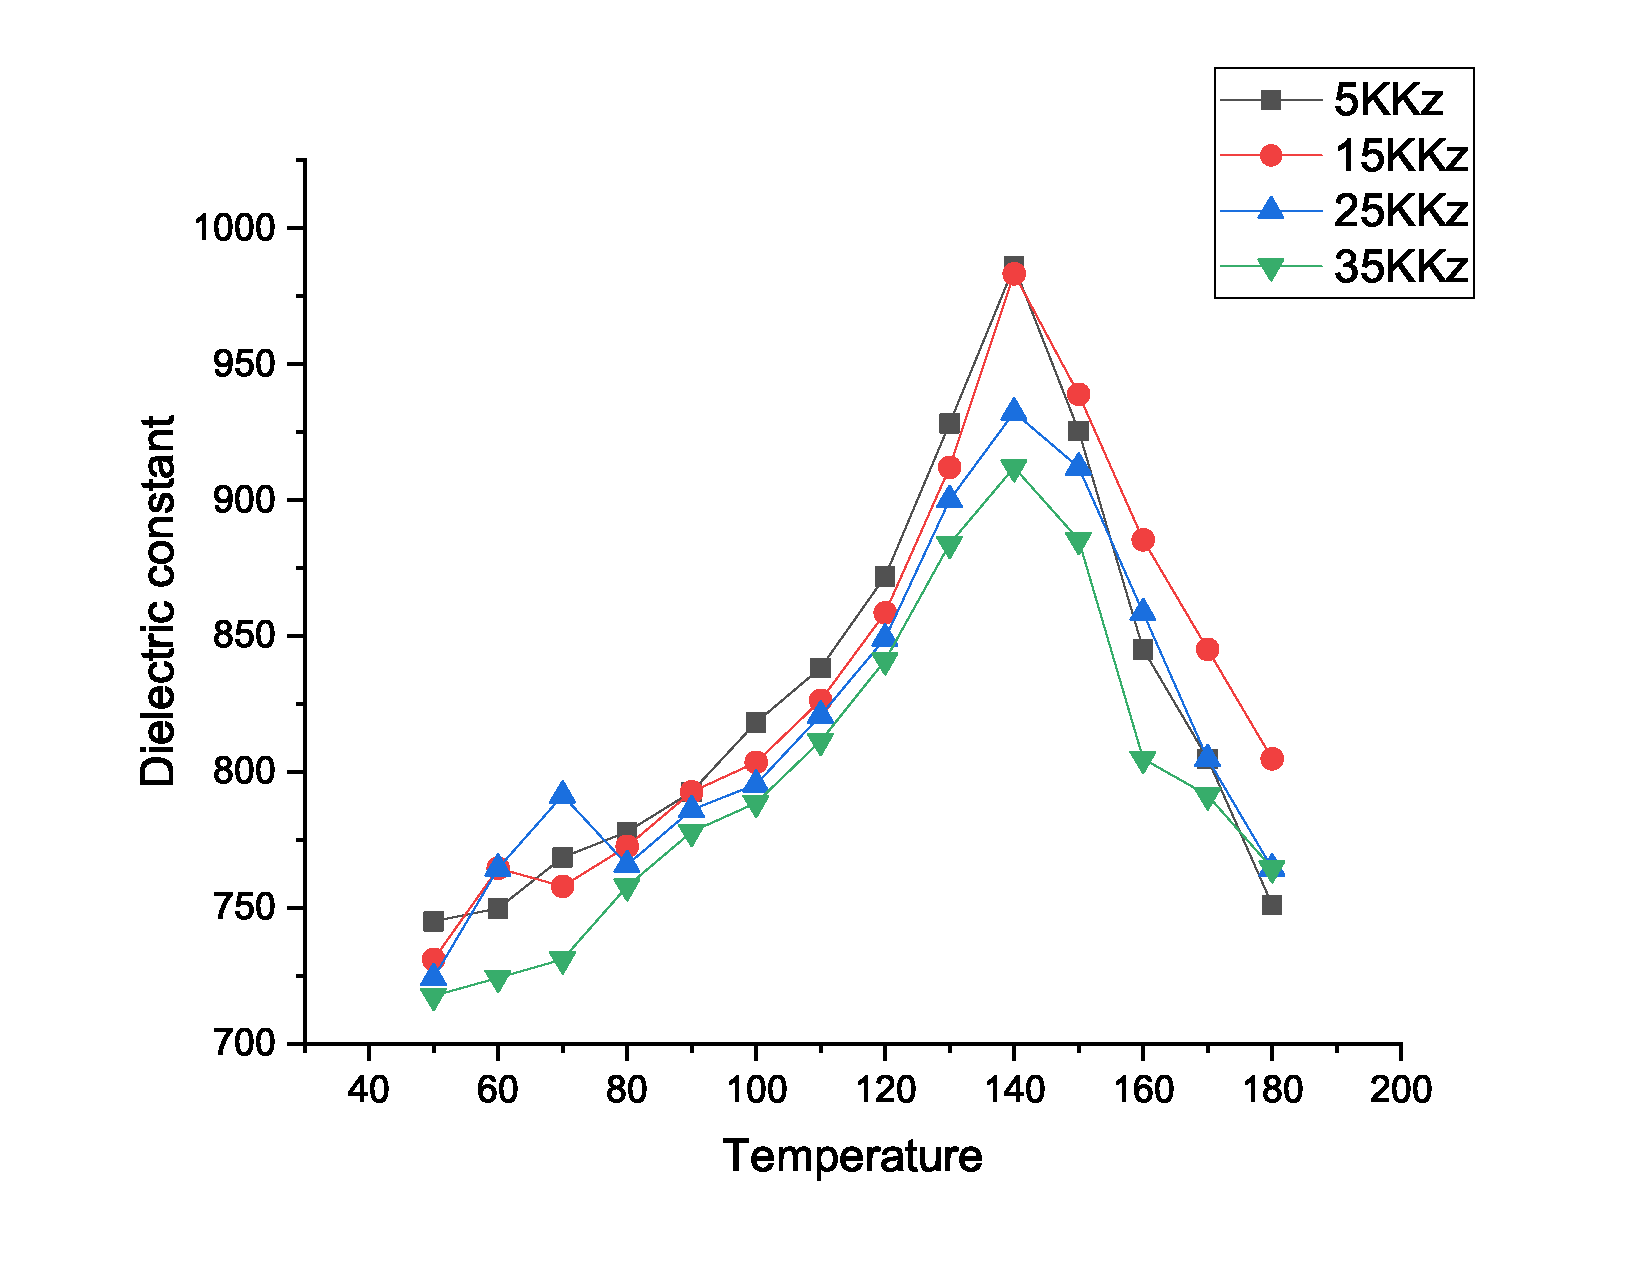
\includegraphics[width=0.8\columnwidth]{images/g5.eps}
			\caption{Dielectric constant vs Temperature T($^\circ C$)}
		\end{figure}
		\subsubsection{Study of diffuseness parameter at a single frequency}
			\begin{table}[H]
    \centering
    \begin{tabular}{|c|c|c|c|c|}
        \hline
        ~ log($\frac{1}{T}$ -$\frac{1}{T_c}$) & log($\frac{1}{\epsilon}$ -$\frac{1}{\epsilon_c}$)                                              \\ \hline
        1.00 & -4.19 & -4.32 & -4.63 & -4.48 \\ \hline
        1.30 & -3.77 & -3.95 & -4.04 & -3.84 \\ \hline
        1.48 & -3.64 & -3.78 & -3.77 & -3.78 \\ \hline
        1.60 & -3.50 & -3.65 & -3.63 & -3.67 \\ \hline
    \end{tabular}
    \caption{Diffuseness
        parameter for $BaTiO_3$ at different temperature  and frequency}
    \label{tab:8}
\end{table}
			\begin{figure}[H]
				\centering
				\label{graph:6}
				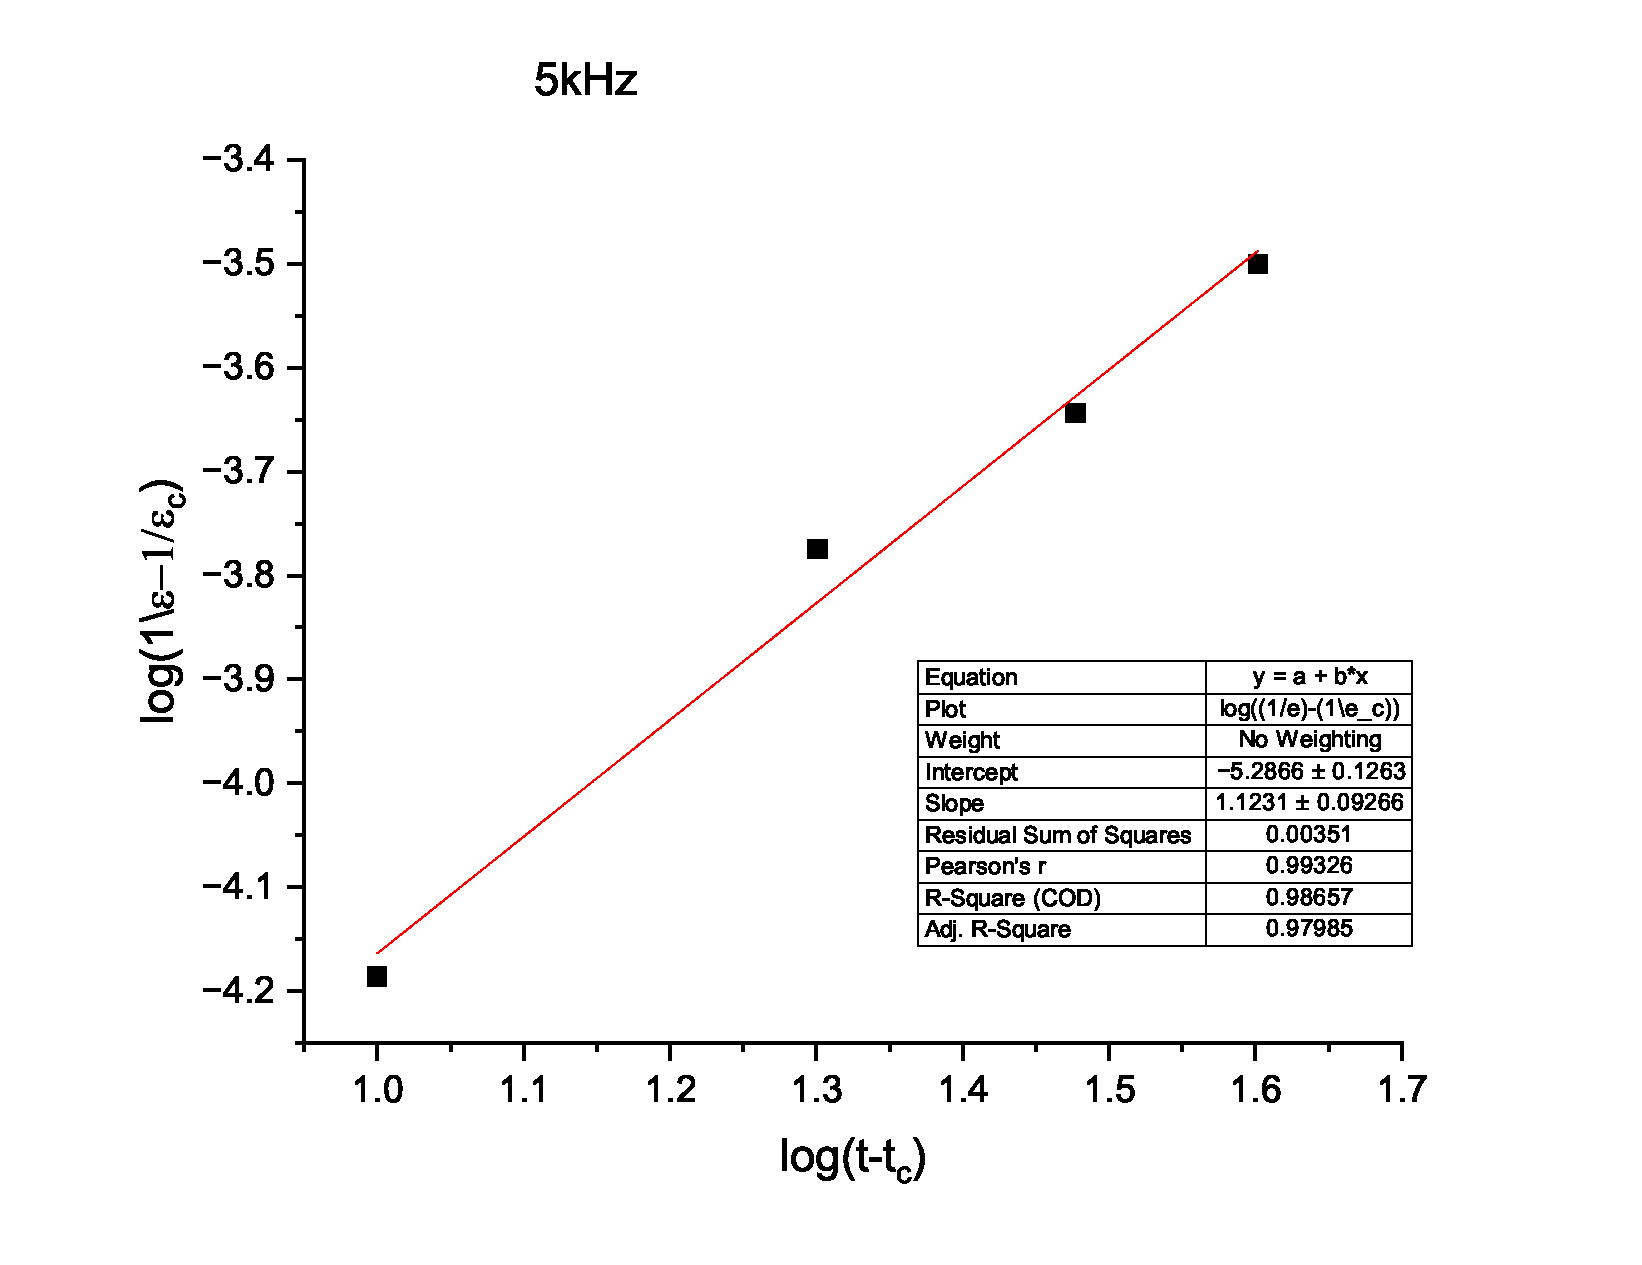
\includegraphics[width=0.8\columnwidth]{images/g6.eps}
				\caption{log($\frac{1}{\epsilon}$ -$\frac{1}{\epsilon_c}$) vs log($\frac{1}{T}$ -$\frac{1}{T_c}$)  at 5KHz}
			\end{figure}
			\begin{figure}[H]
				\centering
				\label{graph:7}
				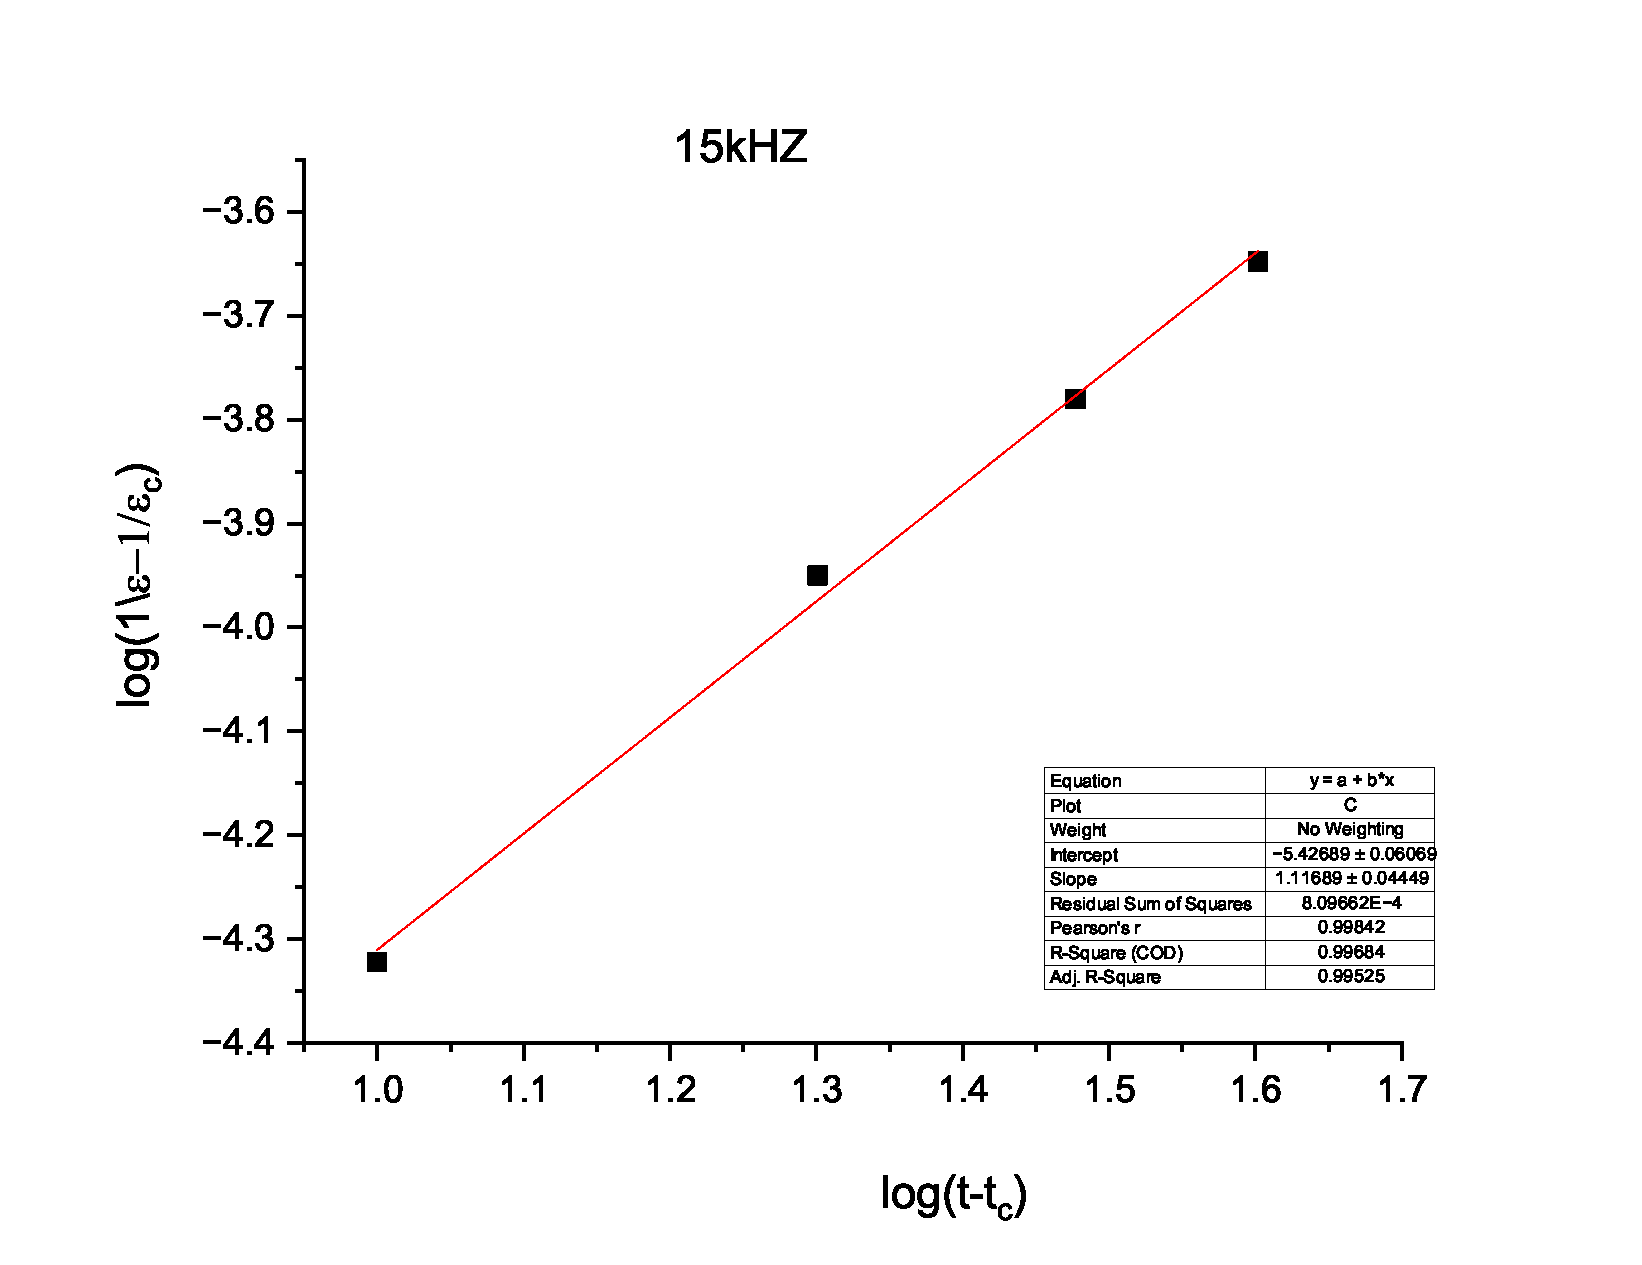
\includegraphics[width=0.8\columnwidth]{images/g7.eps}
				\caption{log($\frac{1}{\epsilon}$ -$\frac{1}{\epsilon_c}$) vs log($\frac{1}{T}$ -$\frac{1}{T_c}$)  at 15KHz}
			\end{figure}
			\begin{figure}[H]
				\centering
				\label{graph:8}
				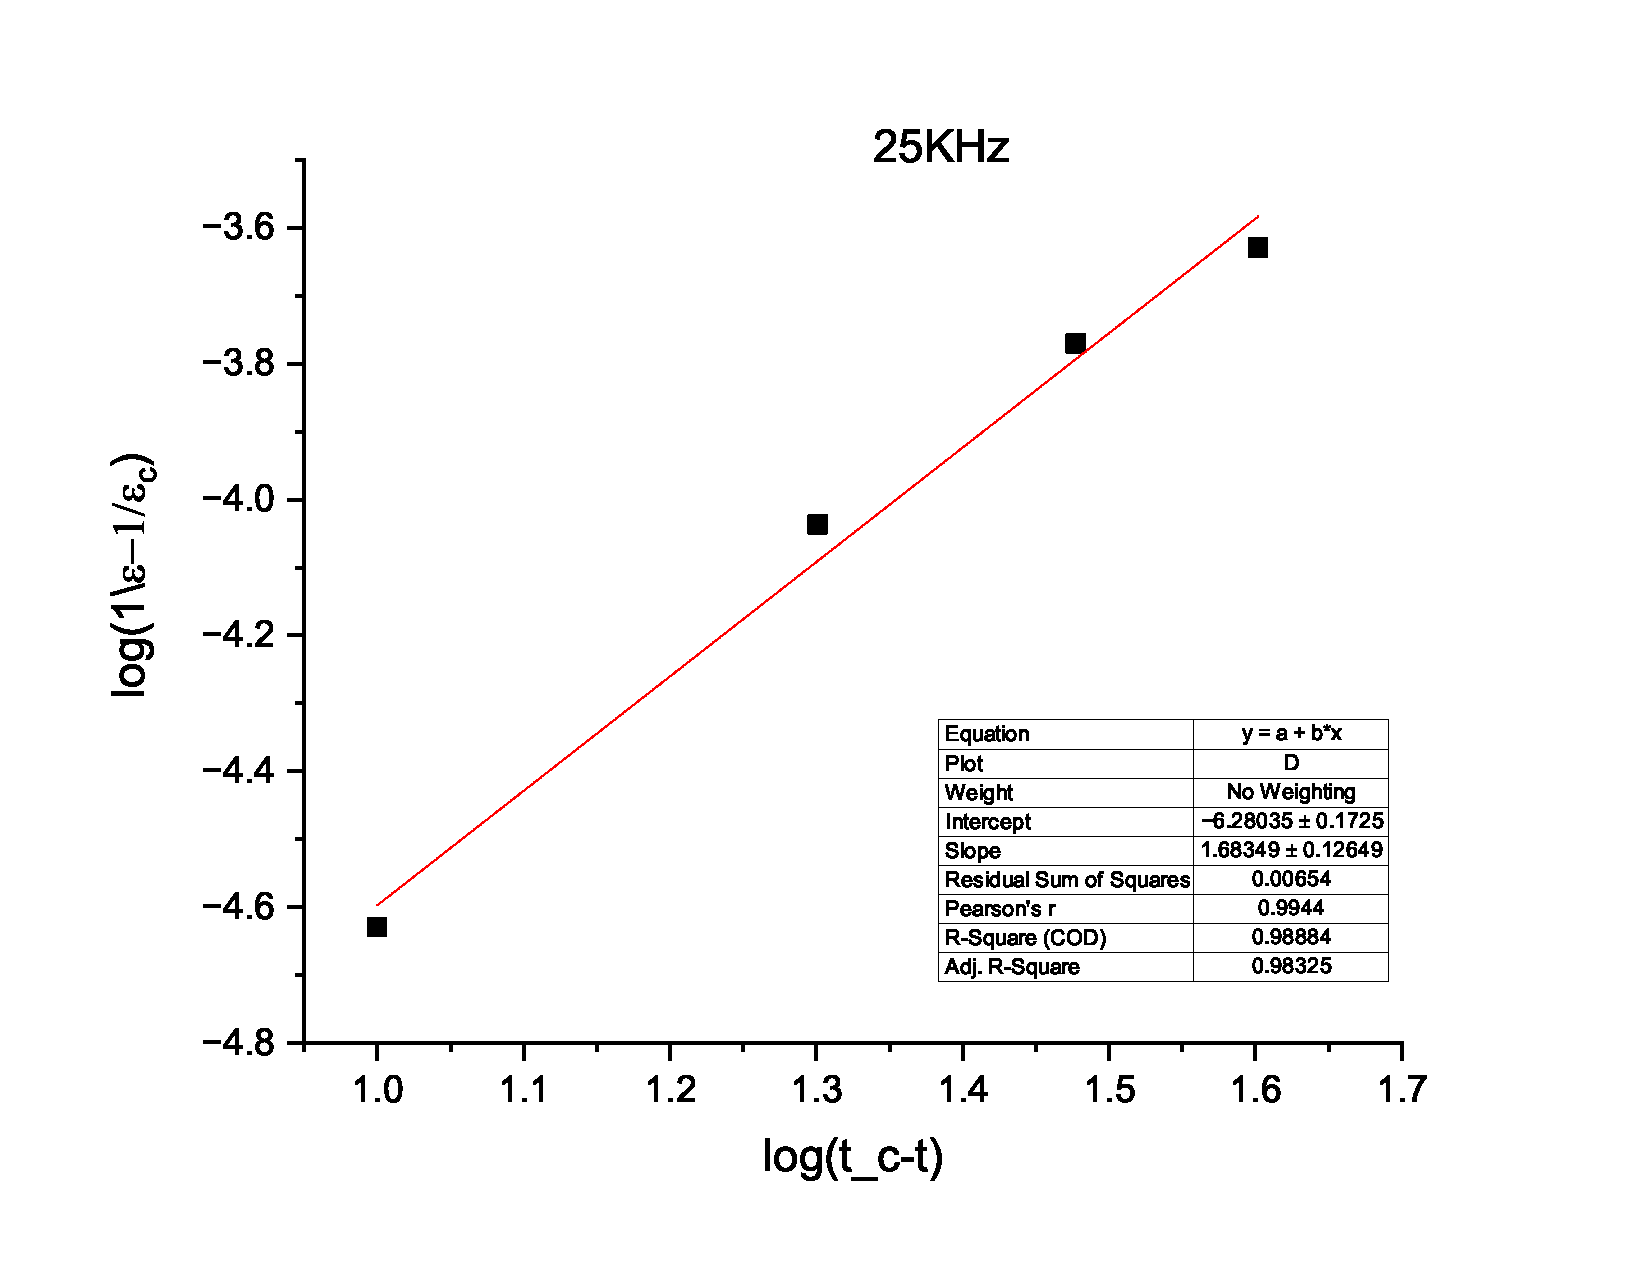
\includegraphics[width=0.8\columnwidth]{images/g8.eps}
				\caption{log($\frac{1}{\epsilon}$ -$\frac{1}{\epsilon_c}$) vs log($\frac{1}{T}$ -$\frac{1}{T_c}$)  at 25KHz}
			\end{figure}
			\begin{figure}[H]
				\centering
				\label{graph:9}
				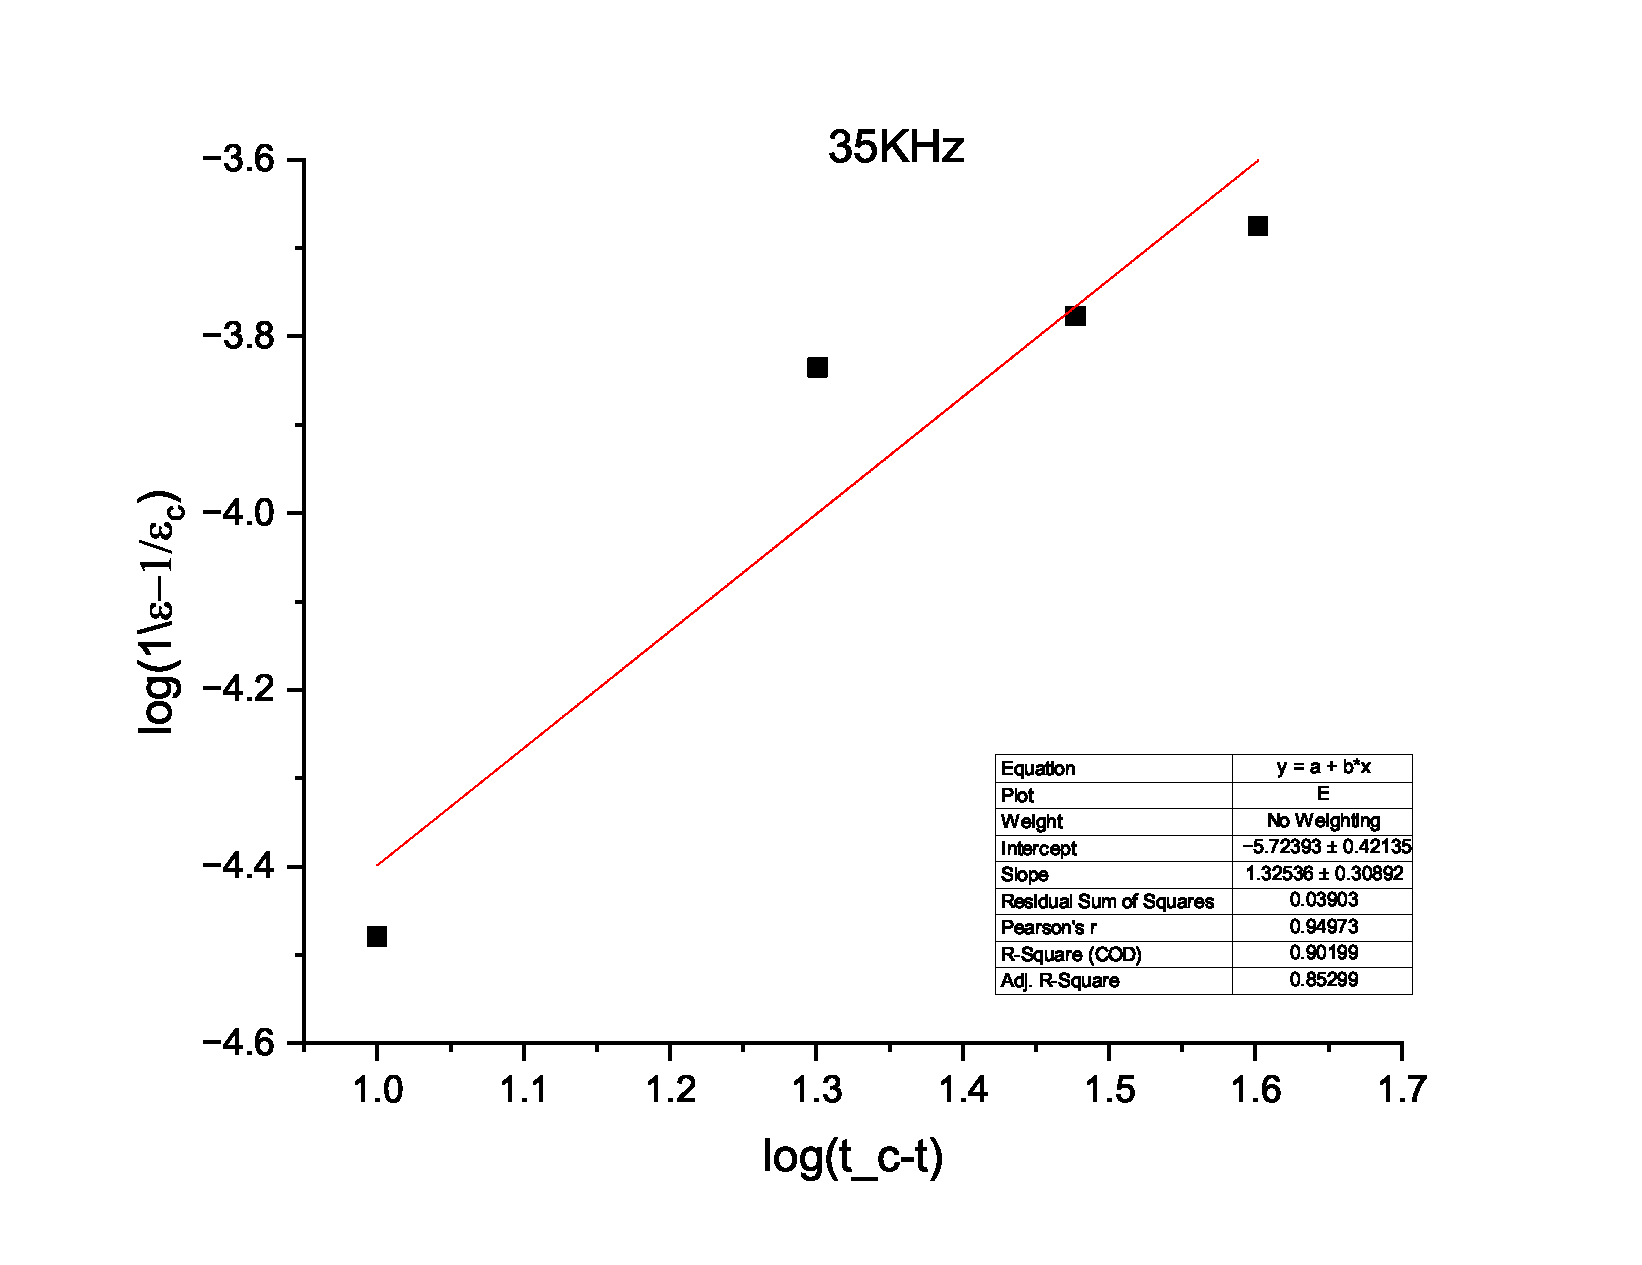
\includegraphics[width=0.8\columnwidth]{images/g9.eps}
				\caption{log($\frac{1}{\epsilon}$ -$\frac{1}{\epsilon_c}$) vs log($\frac{1}{T}$ -$\frac{1}{T_c}$)  at 35KHz}
			\end{figure}
